\documentclass[11pt]{article}
\usepackage[margin=1in]{geometry}
\usepackage{amsmath,amssymb}
\usepackage{booktabs}
\usepackage{enumitem}
\usepackage{xcolor}
\usepackage{tikz}
\usepackage[most]{tcolorbox}
\usepackage[hidelinks]{hyperref}
\usetikzlibrary{arrows.meta,positioning,calc,decorations.pathreplacing,decorations.pathmorphing}

\setlist[itemize]{itemsep=2pt,leftmargin=*}

% ---- palette ----
\definecolor{baseblue}{HTML}{1F4E79}
\definecolor{baseacc}{HTML}{2E86C1}
\definecolor{basegreen}{HTML}{1E8449}
\definecolor{basered}{HTML}{C0392B}
\definecolor{baseorange}{HTML}{E67E22}
\definecolor{baseyellow}{HTML}{F1C40F}

% ---- callout boxes ----
\newtcolorbox{crit}{colback=baseblue!6,colframe=baseblue,fonttitle=\bfseries,
  title=Critical number,boxrule=0.6pt,arc=2pt,left=6pt,right=6pt,top=3pt,bottom=3pt,
  before skip=6pt,after skip=8pt}
\newtcolorbox{means}{colback=basegreen!8,colframe=basegreen,fonttitle=\bfseries,
  title=What it means for Base,boxrule=0.6pt,arc=2pt,left=6pt,right=6pt,top=3pt,bottom=3pt,
  before skip=6pt,after skip=12pt}

\newcommand{\qsec}[1]{\vspace{2pt}\noindent{\large\bfseries\color{baseblue} #1}\par\vspace{2pt}}

\title{\vspace{-1.2cm}\bfseries Can Base's Battery Fleet Be Used to Harm the Grid?\\[2pt]
\large A plain-language security review of the ${\sim}20{,}000$-unit virtual power plant}
\author{}
\date{}

\begin{document}
\maketitle
\vspace{-1.3cm}

\begin{center}
\begin{tcolorbox}[colback=gray!5,colframe=gray!55,width=0.96\linewidth,boxrule=0.5pt,arc=2pt]
\small We stress-tested what someone who seized control of the fleet could do --- to the
Texas grid, to the market price, and to the batteries themselves --- and, more importantly,
what stops them. Everything here runs on public or synthetic models of the grid; no real
circuit is targeted. \textbf{Every risk below is paired with its fix.}
\end{tcolorbox}
\end{center}

% =====================================================================
\qsec{The whole story in one picture}

A battery fleet only gains power over the grid or the price when \textbf{three things line
up at once}: the grid is \emph{already stressed}, many batteries act \emph{in lockstep}, and
\emph{nobody is watching the pattern}. Remove any one and the risk collapses. That single
idea drives every finding.

First, how big is the fleet, really? Elementary arithmetic sets the ceiling:
\[
\underbrace{20{,}000}_{\text{units}}\times\underbrace{20\,\text{kW}}_{\text{each}}
=\;400\,\text{MW},
\qquad
400\,\text{MW}\;\div\;\underbrace{90{,}000\,\text{MW}}_{\text{Texas summer peak}}
\;\approx\;\mathbf{0.4\%}.
\]
And because each battery stores only two hours of energy
($800\,\text{MWh}\div 400\,\text{MW}=2\,\text{h}$), it cannot act for long.

\begin{center}
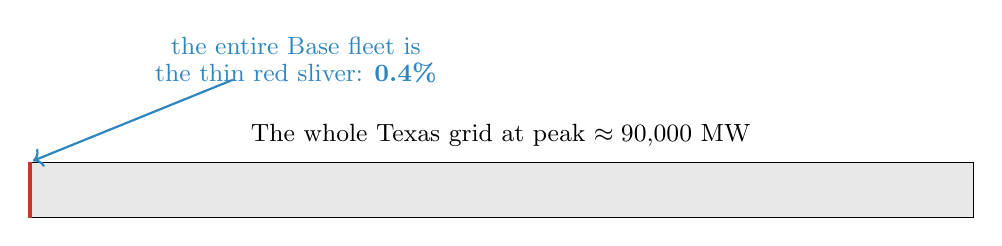
\begin{tikzpicture}[x=1cm,y=1cm]
  \fill[gray!18] (0,0) rectangle (12,0.7);
  \draw (0,0) rectangle (12,0.7);
  \fill[basered] (0,0) rectangle (0.05,0.7); % 0.4% of 12 ~ 0.05
  \node at (6,1.05) {\small The whole Texas grid at peak $\approx 90{,}000$ MW};
  \draw[->,baseacc,thick] (2.6,1.75) -- (0.06,0.72);
  \node[align=center,baseacc] at (3.4,2.0) {\small the entire Base fleet is\\[-2pt]\small the thin red sliver: \textbf{0.4\%}};
\end{tikzpicture}
\end{center}

\begin{crit}
The fleet is \textbf{0.4\%} of the grid and can run for only \textbf{2 hours}. There is no
``crash Texas'' button hiding in it. The real questions are narrower --- and answered below.
\end{crit}

% =====================================================================
\qsec{Question 1 \ \textbullet\ \ Can the fleet crash the grid or the market?}

\textbf{The market price.} Grid price behaves like the curve below: nearly flat in normal
hours, and steep only when supply is scarce. The price you can move equals the \emph{slope}
of this curve times the MW you push:
\[
\Delta\text{price}\;=\;\text{slope}\times\text{MW}.
\]
On real ERCOT data, in calm hours the slope is tiny, so
$0.00025\times400\approx\$0.10$/MWh --- nothing. In scarcity the slope is ${\sim}3{,}000\times$
larger, so $0.79\times400\approx\$300$/MWh (about $13\%$ of a \$2{,}500 price) --- and even
that is hard-capped at the \$5{,}000 offer cap and lasts at most 2 hours.

\begin{center}
\begin{tikzpicture}[x=1cm,y=0.85cm]
  \draw[->] (0,0)--(9.2,0) node[right,font=\scriptsize]{grid load $\to$};
  \draw[->] (0,0)--(0,5) node[above,font=\scriptsize]{price};
  \draw[very thick,baseacc] (0.3,0.35) .. controls (4.5,0.55) and (6.3,0.9) .. (7,1.9)
        .. controls (7.4,3.1) and (7.6,4.4) .. (7.75,4.8);
  \fill (3,0.45) circle (2.2pt); \node[below=1pt,font=\scriptsize] at (3,0.45){calm: flat (no leverage)};
  \fill (7.35,3.4) circle (2.2pt); \node[left=1pt,font=\scriptsize,align=right] at (7.3,3.6){scarcity:\\steep but capped};
\end{tikzpicture}
\end{center}

\begin{crit}
Whole-fleet price impact: \textbf{${\sim}\$0.10$/MWh in calm hours}, at most
\textbf{${\sim}\$300$/MWh ($\approx13\%$) in scarcity}, capped and limited to 2 hours. There
is \textbf{no market crash}.
\end{crit}

\textbf{The physical grid.} A real blackout is not a price event --- it is a \emph{reserve}
event. ERCOT sheds power (rolling blackouts) when its spare capacity (``reserves'') falls to
$1{,}430$ MW. How many batteries would it take to push reserves down to that line?
\[
\text{batteries needed}\;=\;\frac{\text{reserve gap}}{0.04\,\text{MW per battery}}.
\]

\begin{center}
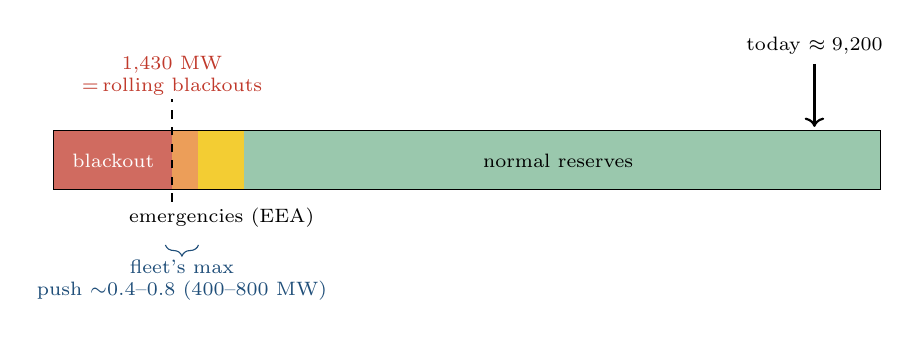
\begin{tikzpicture}[x=1.05cm,y=1cm]
  % zones (1 unit = 1000 MW), 0..10
  \fill[basered!75]   (0,0)     rectangle (1.43,0.75);
  \fill[baseorange!75](1.43,0)  rectangle (1.75,0.75);
  \fill[baseyellow!85](1.75,0)  rectangle (2.30,0.75);
  \fill[basegreen!45] (2.30,0)  rectangle (10,0.75);
  \draw (0,0) rectangle (10,0.75);
  \node[font=\scriptsize,white] at (0.72,0.375){blackout};
  \draw[dashed] (1.43,-0.15)--(1.43,1.15);
  \node[font=\scriptsize,basered,align=center] at (1.43,1.45){$1{,}430$ MW\\=\,rolling blackouts};
  \node[font=\scriptsize] at (2.03,-0.35){emergencies (EEA)};
  \node[font=\scriptsize] at (6.1,0.375){normal reserves};
  % today marker
  \draw[thick,->] (9.2,1.6)--(9.2,0.8); \node[font=\scriptsize,above] at (9.2,1.6){today $\approx 9{,}200$};
  % fleet push bracket near EEA2
  \draw[decorate,decoration={brace,amplitude=4pt},baseblue] (1.75,-0.7)--(1.35,-0.7);
  \node[font=\scriptsize,baseblue,align=center] at (1.55,-1.15){fleet's max\\push ${\sim}0.4$--$0.8$ ($400$--$800$ MW)};
\end{tikzpicture}
\end{center}
\vspace{2pt}

From \emph{today's} healthy reserves that gap is huge:
$(9{,}200-1{,}430)\div0.04\approx\mathbf{195{,}000}$ batteries --- about $10\times$ the whole
fleet. Impossible. But during a \emph{real} emergency (Sept.\ 6, 2023, reserves at $1{,}750$),
the gap is small: $(1{,}750-1{,}430)\div0.04\approx\mathbf{8{,}000}$ batteries --- only $40\%$
of the fleet.

\begin{crit}
To cause rolling blackouts: \textbf{${\sim}195{,}000$ batteries ($10\times$ the fleet) on a
healthy grid} --- impossible; but only \textbf{${\sim}8{,}000$ ($40\%$ of the fleet) on an
already-critical grid}. The fleet becomes dangerous \emph{only} once reserves are already near
empty (below ${\sim}2{,}230$ MW).
\end{crit}

\begin{means}
The fleet cannot crash a healthy grid. The single genuine system risk is \emph{tipping an
already-failing grid}, and one rule removes it: \textbf{batteries must never \emph{charge}
during a grid emergency} --- during scarcity they should discharge to help, never draw power.
\end{means}

% =====================================================================
\qsec{Question 2 \ \textbullet\ \ How many batteries overload one neighborhood?}

The reachable damage is \emph{local}: too many batteries behind one street transformer,
all pushing together, overload the local wires. The threshold is simple to size:
\[
\frac{\text{local transformer limit}}{\text{battery size}}
\;\approx\;\frac{3\,\text{MW}}{20\,\text{kW}}\;\approx\;\mathbf{108}\ \text{batteries.}
\]

\begin{center}
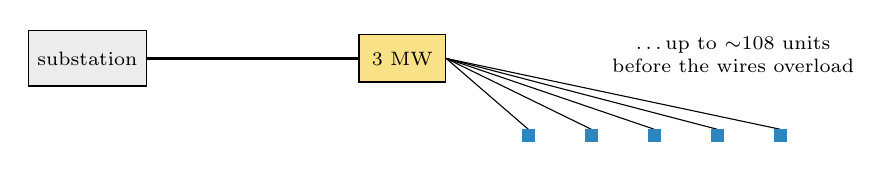
\begin{tikzpicture}[x=1cm,y=1cm]
  \node[draw,fill=gray!15,minimum width=1.4cm,minimum height=0.7cm,font=\scriptsize] (sub) at (0,0){substation};
  \node[draw,fill=baseyellow!50,minimum width=1.1cm,minimum height=0.6cm,font=\scriptsize] (tx) at (4,0){3 MW};
  \draw[very thick] (sub.east)--(tx.west);
  \foreach \i in {0,...,4}{
    \draw (tx.east)--(5.6+\i*0.8,-0.9);
    \fill[baseacc] (5.6+\i*0.8-0.08,-1.06) rectangle ++(0.16,0.16);
  }
  \node[font=\scriptsize,align=center] at (8.2,0.05){\dots up to ${\sim}108$ units\\before the wires overload};
\end{tikzpicture}
\end{center}

\begin{crit}
${\sim}\mathbf{108}$ co-located batteries (about $2$ MW) overload a local feeder ---
\textbf{hundreds, not tens of thousands.}
\end{crit}

\begin{means}
Physical risk is a neighborhood problem, not a statewide one. \textbf{Cap how many Base
batteries sit behind one transformer} (a safe limit is ${\sim}75$), and block whole streets
from being commanded in perfect lockstep.
\end{means}

% =====================================================================
\qsec{Question 3 \ \textbullet\ \ Could someone quietly bleed money or wear out batteries over months?}

A patient attacker could nudge dispatch a tiny bit every day --- too small to notice in any
single snapshot --- and let the cost pile up. Left unwatched for six months that could total
tens of millions. The defense is a \emph{trend} alarm (it adds up small deviations over time),
and it has a neat property: a stealthier attacker does less damage per day but takes
proportionally longer to catch, so the \textbf{total} damage before detection is \emph{bounded}
no matter how slow they go.

\begin{center}
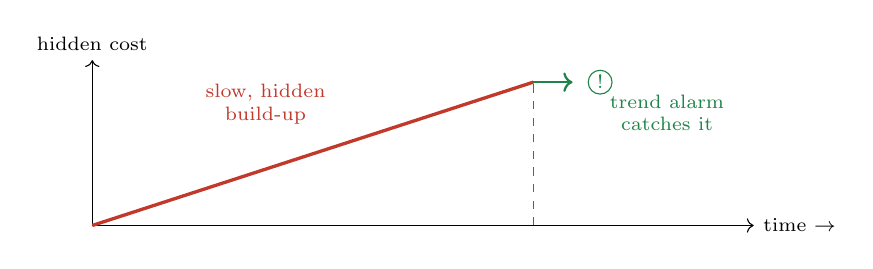
\begin{tikzpicture}[x=1cm,y=0.7cm]
  \draw[->](0,0)--(8.4,0) node[right,font=\scriptsize]{time $\to$};
  \draw[->](0,0)--(0,3) node[above,font=\scriptsize]{hidden cost};
  \draw[very thick,basered] (0,0)--(5.6,2.6);
  \node[font=\scriptsize,basered,align=center] at (2.2,2.2){slow, hidden\\build-up};
  \draw[thick,basegreen,->] (5.6,2.6)--(6.1,2.6);
  \node[draw,circle,basegreen,font=\scriptsize,inner sep=1.2pt] at (6.45,2.6){!};
  \node[font=\scriptsize,basegreen,align=center] at (7.3,2.05){trend alarm\\catches it};
  \draw[dashed,basegreen] (5.6,0)--(5.6,2.6);
\end{tikzpicture}
\end{center}

\begin{crit}
Undetected, a slow attack could add \textbf{\$18--117M over six months}. With a trend
(CUSUM) monitor, total damage before detection is \textbf{capped at ${\sim}\$7M} --- for any
stealth level.
\end{crit}

\begin{means}
Per-snapshot checks are not enough on their own. \textbf{Add a cumulative trend monitor};
then patient, low-and-slow attacks simply cannot win.
\end{means}

% =====================================================================
\qsec{Question 4 \ \textbullet\ \ Could a hacker physically destroy the batteries?}

Yes --- the sharpest hardware attack is \textbf{constant switching}: flipping each unit
between charge and discharge as fast as possible. The power electronics survive only a fixed
number of such flips, so their life is simple arithmetic:
\[
\text{life}\;=\;\frac{\text{flips the inverter can survive}}{\text{flips per day}}.
\]
Normal operation flips ${\sim}6$ times a day (life $>250$ years). Constant flipping
($86{,}400$ times a day) destroys the inverter in about \textbf{6 days}.

\begin{center}
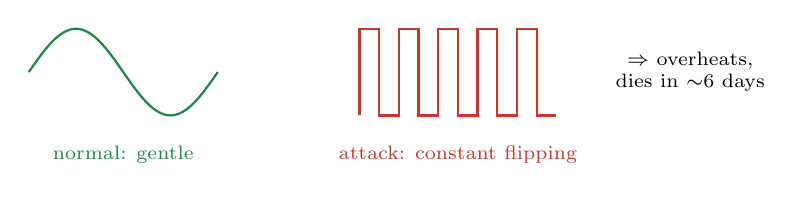
\begin{tikzpicture}[x=1cm,y=0.55cm]
  % gentle wave (normal)
  \draw[thick,basegreen] (0,1) sin (0.6,2) cos (1.2,1) sin (1.8,0) cos (2.4,1);
  \node[font=\scriptsize,basegreen] at (1.2,-0.9){normal: gentle};
  % rapid square wave (attack)
  \begin{scope}[xshift=4.2cm]
   \draw[thick,basered] (0,0)--(0,2)--(0.25,2)--(0.25,0)--(0.5,0)--(0.5,2)--(0.75,2)--(0.75,0)
        --(1,0)--(1,2)--(1.25,2)--(1.25,0)--(1.5,0)--(1.5,2)--(1.75,2)--(1.75,0)--(2,0)--(2,2)--(2.25,2)--(2.25,0)--(2.5,0);
   \node[font=\scriptsize,basered] at (1.25,-0.9){attack: constant flipping};
  \end{scope}
  \node[font=\scriptsize,align=center] at (8.4,1){$\Rightarrow$ overheats,\\dies in ${\sim}6$ days};
\end{tikzpicture}
\end{center}

\begin{crit}
Constant switching can destroy a unit's power electronics in \textbf{${\sim}6$ days}.
A firmware cap of \textbf{$\le48$ direction-changes per day} restores ${\sim}30$-year life.
\end{crit}

\begin{means}
Add a \textbf{firmware limit on how often (and how fast) a battery may reverse direction}.
It is cheap, and an abnormal switching rate is glaringly obvious in telemetry.
\end{means}

% =====================================================================
\qsec{Question 5 \ \textbullet\ \ What single thing catches all of this?}

Every attack above needs \textbf{many batteries doing the same thing at the same time}.
Normal batteries are diverse --- their actions point in different directions and cancel out.
So one number --- \emph{how alike the batteries are behaving} (their correlation) --- flags any
coordinated attack, whatever its goal.

\begin{center}
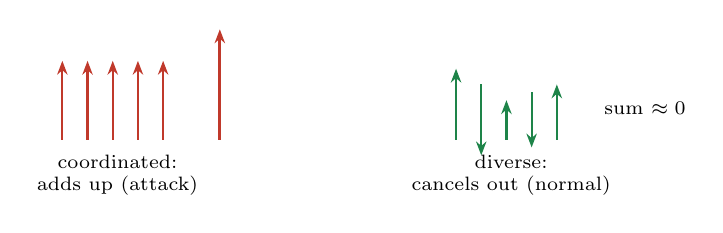
\begin{tikzpicture}[x=1cm,y=1cm,>={Stealth[length=5pt]}]
  % coordinated
  \foreach \i in {0,...,4}{\draw[->,thick,basered] (\i*0.32,0)--(\i*0.32,1);}
  \draw[->,very thick,basered] (2.0,0)--(2.0,1.4);
  \node[font=\scriptsize,align=center] at (0.7,-0.45){coordinated:\\adds up (attack)};
  % independent
  \begin{scope}[xshift=5cm]
    \draw[->,thick,basegreen](0,0)--(0,0.9);
    \draw[->,thick,basegreen](0.32,0.7)--(0.32,-0.2);
    \draw[->,thick,basegreen](0.64,0)--(0.64,0.5);
    \draw[->,thick,basegreen](0.96,0.6)--(0.96,-0.1);
    \draw[->,thick,basegreen](1.28,0)--(1.28,0.7);
    \node[font=\scriptsize] at (2.4,0.4){sum $\approx 0$};
    \node[font=\scriptsize,align=center] at (0.7,-0.45){diverse:\\cancels out (normal)};
  \end{scope}
\end{tikzpicture}
\end{center}

\begin{crit}
Normal cross-battery correlation is ${\approx}0$; a coordinated attack drives it up. A single
alarm --- \textbf{correlation $>0.2$ over a day} --- catches price, grid, degradation, and
switching attacks alike.
\end{crit}

\begin{means}
\textbf{One cheap monitor} (are the batteries suspiciously in sync?) covers essentially every
threat at once, because coordination is the common ingredient of all of them.
\end{means}

% =====================================================================
\qsec{What Base should do}

\begin{enumerate}[leftmargin=1.4em,itemsep=2pt]
\item \textbf{No charging during grid emergencies.} When ERCOT reserves are low, batteries
support the grid --- they never draw power. (Removes the only real system-crash path.)
\item \textbf{Cap batteries per transformer} (${\sim}75$), and forbid whole-street lockstep
commands. (Removes local overloads.)
\item \textbf{Watch coordination.} Alarm when batteries behave too alike (correlation $>0.2$),
plus a slow-trend monitor. (Catches price, degradation, and stealth attacks.)
\item \textbf{Firmware guardrails.} Cap direction-changes ($\le48$/day) and ramp speed; keep
charge/discharge within the unit's rating and above a $10\%$ floor. (Protects the hardware.)
\item \textbf{Focus monitoring on scarcity windows}, when the only real leverage exists.
\end{enumerate}

\begin{tcolorbox}[colback=baseblue!7,colframe=baseblue,boxrule=0.7pt,arc=2pt,
  title=Bottom line,fonttitle=\bfseries,coltitle=white]
There is no ``crash Texas'' button in this fleet: at $0.4\%$ of the grid and two hours of
energy, it cannot topple a healthy system or the market. The genuine risks are narrow and
familiar --- \emph{local} overloads, \emph{tipping an already-failing grid}, slow hidden
waste, and hardware wear --- and every one is \textbf{bounded, cheaply detectable, and closed
by the five steps above}. The same analysis that measures the fleet's \emph{value} to Base
also measures an attacker's \emph{ceiling} --- and that ceiling is low.
\end{tcolorbox}

\vfill
\noindent{\footnotesize Based on public ERCOT market and reserve data and published,
synthetic grid models; full methods, figures, and formulas in the accompanying technical
report. Defensive framing throughout: no real circuit is modeled or targeted.}

\end{document}
